Robots were created in Wave with the intention to be able to act exactly as an actual human participant. Revisiting Figure \ref{fig:wave_structure} we can understand how robots can participate: They are invited to the Wave by inserting their unique identifier. They will aprear as invited without any apparent indication that they are a robot. Robots can make changes to the Wave such as creating a new blip, editing them, changing annotations...\\[.2cm]
In order to be able to interact with Wave it is necessary to register the robot with the Wave server where the robot will be run. For example, for the Kune node kune.cc, go to \url{http://kune.cc/robot/register/create} and you will be prompted with the screen shown in Figure \ref{fig:robot_register}.
\begin{figure}[H]
  \center
    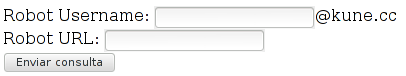
\includegraphics[keepaspectratio, scale=0.6]{Media/Captures/Wave/RegisterRobot.png}
  \caption{Robot Registration Screen}
  \label{fig:robot_register}
\end{figure}
As username set the name you wish to give your robot, it should be a free name in the server, as names are unique. In the URL enter the URL where the gadget will be launched, it should be an URL reachable from within the Wave server. After sending the data you will receive a Consumer Token matching the name you entered, and a Consumer Token Secret: a secret key you will need to use to authenticate with OAuth and guarantee the identity of your robot.\\[.2cm]
There is no equivalent to the tester mode from GWT, but running a server for the robots is easy enough so it is not a hassle. Using Maven plus Jetty you can set the Maven goal to \verb|jetty:run| and the robot will be run.\\[.2cm]
Robots do basically two thins: Act when needed, and react to events. Acting means modifying the documents, creating new blips... And receiving events means a callback will be made to the robot when something from an external action happens on the Wave. The kind of events that are notified to the robot are the following:
\begin{itemize}
  \item WaveletBlipCreated: Triggered when a new blip is created.
  \item WaveletBlipRemoved: Triggered when a blip is deleted.
  \item WaveletParticipantsChanged: Triggered when a participant is added or removed.
  \item WaveletSelfAdded: Triggered when the own robot is added as a participant.
  \item WaveletSelfRemoved: Triggered when the own robot is removed as a participant.
  \item DocumentChanged: Triggered when the text of a document changes.
  \item AnnotatedTextChanged: Triggered when the annotations of a document change.
\end{itemize}
There are other events documented such as GadgetStateChanged or WaveletTagsChanged, which even though available through the Robots API will not be triggered on the server, and therefore never received.

\subsection{Colorizer Robot}
Again, text communications gets in the way of collaboration in some aspects. When working between several people it is sometimes necessary to talk about some aspect of the work they disagree in. In plain text, when there are more than two collaborators, there is no way to know who edited what, so those kind of issues can't be addressed personally. A robot is needed in order to know when and what changes are being made.

\subsubsection{State of the Art}
In Wave it is possible to see who has participated in a blip as shown in Figure \ref{fig:participants}, but it is not possible to see exactly what that participant has modified what part of the document.
\begin{figure}[H]
  \center
    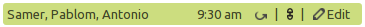
\includegraphics[keepaspectratio, scale=0.7]{Media/Captures/Wave/Participants.png}
  \caption{Blip Participants in Kune}
  \label{fig:participants}
\end{figure}
The other thing Wave does to try to keep people informed on when changes happen, is to highlight the changes that just happened and write the author's name next to it, as shown in Figure \ref{fig:participants2}. The problem is it is not permanent, so you only realize of the change if you were already looking at the content being changed.
\begin{figure}[H]
  \center
    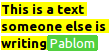
\includegraphics[keepaspectratio, scale=0.7]{Media/Captures/Wave/Participants2.png}
  \caption{Change Highlighting in Kune}
  \label{fig:participants2}
\end{figure}
Also, this extension is heavily inspired in Pads, services like PiratePad, Etherpad, TitanPad and many others, that offer an online collaboration tool that allows to concurrently write plain-text documents. They show a specific color for each participant to quickly see who edited what. TitanPad in Figure \ref{fig:titanpad}, even though not the only, has the capability to show a timeline and revisit past states of the Pad, so no information is lost even after being modified.
\begin{figure}[h]
  \center
    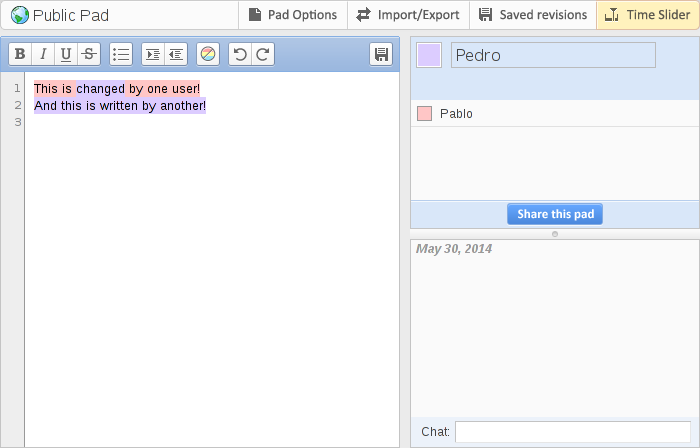
\includegraphics[keepaspectratio, scale=0.4]{Media/Captures/Soa/TitanPad.png}
  \caption{TitanPad}
  \label{fig:titanpad}
\end{figure}

\subsubsection{Results}
This extension, in the shape of a robot, goes around that problem by assigning a color to each participant, and painting the background of the text that participant edits. The result can be seen in Figure \ref{fig:colorizer_editions}. It also keeps track of who has each color and puts it in a blip under the main blip of the wave, as seen in Figure \ref{fig:colorizer_editors}. It is also possible to get around the colorizing of any given blip by starting it with \verb|@Robot clear annotations|, being ``Robot'' the actual name of the robot that it was registered with.\\[.2cm]
\begin{figure}[H]
  \center
    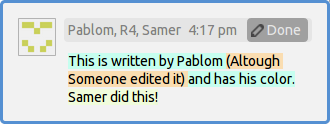
\includegraphics[keepaspectratio, scale=0.8]{Media/Captures/Extensions/Colorizer/ColorizerEditions.png}
  \caption{Colorizer Robot Colors}
  \label{fig:colorizer_editions}
\end{figure}
\begin{figure}[h]
  \center
    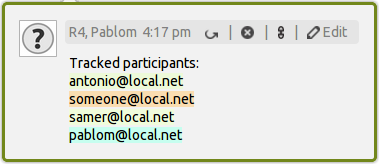
\includegraphics[keepaspectratio, scale=0.7]{Media/Captures/Extensions/Colorizer/ColorizerEditors.png}
  \caption{Colorizer Robot Tracking Participants}
  \label{fig:colorizer_editors}
\end{figure}
The way to make the background of the text be of a specific color is by changing the annotations of the document. Annotations in Wave are tags affecting a range of text and altering its properties, but they don't affect the text itself. Annotations are also able to be transmitted through the Federation Protocol. Every annotation is defined by a name (What it does), a range (What characters of text it affects), and a value (What value should that annotation take on that range). There are annotations for text size, links, language... For this robot specifically the annotation \verb|style/backgroundColor| is the one being set in the changed text.\\[.2cm]
The way to know when the changes happen is by subscribing th the DocumentChanged event explained before. This event will be triggered anytime anyone modifies the tex.\\[.2cm]
\begin{figure}[H]
  \center
    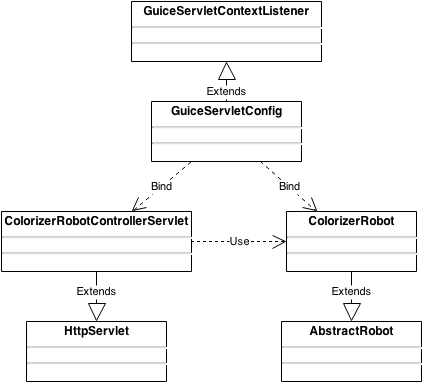
\includegraphics[keepaspectratio, scale=0.5]{Media/Diagrams/Robot/Colorizer.png}
  \caption{Colorizer Robot Class Diagram}
  \label{fig:colorizer_diagram}
\end{figure}
That only leaves one task left: The DocumentChanged event tells us the document has changed, but not what part changed or how it changed, so it is up to us to extract that information. To achieve it Google's google-diff-match-patch, a Java library that is able to extract the difference between two chunks of plain text. Every time the document is changed, the difference with the last version is calculated, and the new content is attributed to the participant that changed it.\\[.2cm]
Figure \ref{fig:colorizer_diagram} represents the class structure of the Colorizer Robot. The HttpServlet is the responsible of receiving the communication from the Wave Protocol. The ColorizerRobot sets up the OAuth authentication with the token received when registering the robot. Also, thanks to the AbstractGadget class it is registered to receive all the events. The GuiceServletConfig binds the necessary dependencies together.
